% Options for packages loaded elsewhere
\PassOptionsToPackage{unicode}{hyperref}
\PassOptionsToPackage{hyphens}{url}
%
\documentclass[
]{article}
\usepackage{amsmath,amssymb}
\usepackage{iftex}
\ifPDFTeX
  \usepackage[T1]{fontenc}
  \usepackage[utf8]{inputenc}
  \usepackage{textcomp} % provide euro and other symbols
\else % if luatex or xetex
  \usepackage{unicode-math} % this also loads fontspec
  \defaultfontfeatures{Scale=MatchLowercase}
  \defaultfontfeatures[\rmfamily]{Ligatures=TeX,Scale=1}
\fi
\usepackage{lmodern}
\ifPDFTeX\else
  % xetex/luatex font selection
\fi
% Use upquote if available, for straight quotes in verbatim environments
\IfFileExists{upquote.sty}{\usepackage{upquote}}{}
\IfFileExists{microtype.sty}{% use microtype if available
  \usepackage[]{microtype}
  \UseMicrotypeSet[protrusion]{basicmath} % disable protrusion for tt fonts
}{}
\makeatletter
\@ifundefined{KOMAClassName}{% if non-KOMA class
  \IfFileExists{parskip.sty}{%
    \usepackage{parskip}
  }{% else
    \setlength{\parindent}{0pt}
    \setlength{\parskip}{6pt plus 2pt minus 1pt}}
}{% if KOMA class
  \KOMAoptions{parskip=half}}
\makeatother
\usepackage{xcolor}
\usepackage[margin=1in]{geometry}
\usepackage{color}
\usepackage{fancyvrb}
\newcommand{\VerbBar}{|}
\newcommand{\VERB}{\Verb[commandchars=\\\{\}]}
\DefineVerbatimEnvironment{Highlighting}{Verbatim}{commandchars=\\\{\}}
% Add ',fontsize=\small' for more characters per line
\usepackage{framed}
\definecolor{shadecolor}{RGB}{248,248,248}
\newenvironment{Shaded}{\begin{snugshade}}{\end{snugshade}}
\newcommand{\AlertTok}[1]{\textcolor[rgb]{0.94,0.16,0.16}{#1}}
\newcommand{\AnnotationTok}[1]{\textcolor[rgb]{0.56,0.35,0.01}{\textbf{\textit{#1}}}}
\newcommand{\AttributeTok}[1]{\textcolor[rgb]{0.13,0.29,0.53}{#1}}
\newcommand{\BaseNTok}[1]{\textcolor[rgb]{0.00,0.00,0.81}{#1}}
\newcommand{\BuiltInTok}[1]{#1}
\newcommand{\CharTok}[1]{\textcolor[rgb]{0.31,0.60,0.02}{#1}}
\newcommand{\CommentTok}[1]{\textcolor[rgb]{0.56,0.35,0.01}{\textit{#1}}}
\newcommand{\CommentVarTok}[1]{\textcolor[rgb]{0.56,0.35,0.01}{\textbf{\textit{#1}}}}
\newcommand{\ConstantTok}[1]{\textcolor[rgb]{0.56,0.35,0.01}{#1}}
\newcommand{\ControlFlowTok}[1]{\textcolor[rgb]{0.13,0.29,0.53}{\textbf{#1}}}
\newcommand{\DataTypeTok}[1]{\textcolor[rgb]{0.13,0.29,0.53}{#1}}
\newcommand{\DecValTok}[1]{\textcolor[rgb]{0.00,0.00,0.81}{#1}}
\newcommand{\DocumentationTok}[1]{\textcolor[rgb]{0.56,0.35,0.01}{\textbf{\textit{#1}}}}
\newcommand{\ErrorTok}[1]{\textcolor[rgb]{0.64,0.00,0.00}{\textbf{#1}}}
\newcommand{\ExtensionTok}[1]{#1}
\newcommand{\FloatTok}[1]{\textcolor[rgb]{0.00,0.00,0.81}{#1}}
\newcommand{\FunctionTok}[1]{\textcolor[rgb]{0.13,0.29,0.53}{\textbf{#1}}}
\newcommand{\ImportTok}[1]{#1}
\newcommand{\InformationTok}[1]{\textcolor[rgb]{0.56,0.35,0.01}{\textbf{\textit{#1}}}}
\newcommand{\KeywordTok}[1]{\textcolor[rgb]{0.13,0.29,0.53}{\textbf{#1}}}
\newcommand{\NormalTok}[1]{#1}
\newcommand{\OperatorTok}[1]{\textcolor[rgb]{0.81,0.36,0.00}{\textbf{#1}}}
\newcommand{\OtherTok}[1]{\textcolor[rgb]{0.56,0.35,0.01}{#1}}
\newcommand{\PreprocessorTok}[1]{\textcolor[rgb]{0.56,0.35,0.01}{\textit{#1}}}
\newcommand{\RegionMarkerTok}[1]{#1}
\newcommand{\SpecialCharTok}[1]{\textcolor[rgb]{0.81,0.36,0.00}{\textbf{#1}}}
\newcommand{\SpecialStringTok}[1]{\textcolor[rgb]{0.31,0.60,0.02}{#1}}
\newcommand{\StringTok}[1]{\textcolor[rgb]{0.31,0.60,0.02}{#1}}
\newcommand{\VariableTok}[1]{\textcolor[rgb]{0.00,0.00,0.00}{#1}}
\newcommand{\VerbatimStringTok}[1]{\textcolor[rgb]{0.31,0.60,0.02}{#1}}
\newcommand{\WarningTok}[1]{\textcolor[rgb]{0.56,0.35,0.01}{\textbf{\textit{#1}}}}
\usepackage{graphicx}
\makeatletter
\def\maxwidth{\ifdim\Gin@nat@width>\linewidth\linewidth\else\Gin@nat@width\fi}
\def\maxheight{\ifdim\Gin@nat@height>\textheight\textheight\else\Gin@nat@height\fi}
\makeatother
% Scale images if necessary, so that they will not overflow the page
% margins by default, and it is still possible to overwrite the defaults
% using explicit options in \includegraphics[width, height, ...]{}
\setkeys{Gin}{width=\maxwidth,height=\maxheight,keepaspectratio}
% Set default figure placement to htbp
\makeatletter
\def\fps@figure{htbp}
\makeatother
\setlength{\emergencystretch}{3em} % prevent overfull lines
\providecommand{\tightlist}{%
  \setlength{\itemsep}{0pt}\setlength{\parskip}{0pt}}
\setcounter{secnumdepth}{-\maxdimen} % remove section numbering
\ifLuaTeX
  \usepackage{selnolig}  % disable illegal ligatures
\fi
\usepackage{bookmark}
\IfFileExists{xurl.sty}{\usepackage{xurl}}{} % add URL line breaks if available
\urlstyle{same}
\hypersetup{
  pdftitle={Proyecto\_RNAseq},
  pdfauthor={Karla Ximena González Platas},
  hidelinks,
  pdfcreator={LaTeX via pandoc}}

\title{Proyecto\_RNAseq}
\usepackage{etoolbox}
\makeatletter
\providecommand{\subtitle}[1]{% add subtitle to \maketitle
  \apptocmd{\@title}{\par {\large #1 \par}}{}{}
}
\makeatother
\subtitle{Análisis de Expresión Diferencial}
\author{Karla Ximena González Platas}
\date{2025-02-05}

\begin{document}
\maketitle

{
\setcounter{tocdepth}{2}
\tableofcontents
}
\subsection{Introducción}\label{introducciuxf3n}

\subsection{Instalar y cargas
paquetes}\label{instalar-y-cargas-paquetes}

\begin{Shaded}
\begin{Highlighting}[]
\CommentTok{\# Cargar el paquete de R que incluye a SummarizedExperiment y todas las demás dependencias}
\FunctionTok{library}\NormalTok{(}\StringTok{"recount3"}\NormalTok{)}
\FunctionTok{library}\NormalTok{(}\StringTok{"limma"}\NormalTok{)}
\FunctionTok{library}\NormalTok{(}\StringTok{"edgeR"}\NormalTok{)}
\end{Highlighting}
\end{Shaded}

\subsection{Selección de Proyecto}\label{selecciuxf3n-de-proyecto}

\begin{Shaded}
\begin{Highlighting}[]
\CommentTok{\# Obtener la lista de proyectos disponibles }
\NormalTok{human\_projects }\OtherTok{\textless{}{-}} \FunctionTok{available\_projects}\NormalTok{()}
\end{Highlighting}
\end{Shaded}

\begin{verbatim}
## 2025-02-05 23:17:32.411146 caching file sra.recount_project.MD.gz.
\end{verbatim}

\begin{verbatim}
## 2025-02-05 23:17:33.344082 caching file gtex.recount_project.MD.gz.
\end{verbatim}

\begin{verbatim}
## 2025-02-05 23:17:33.948647 caching file tcga.recount_project.MD.gz.
\end{verbatim}

\begin{Shaded}
\begin{Highlighting}[]
\CommentTok{\# Ver los proyectos disponibles}
\FunctionTok{dim}\NormalTok{(human\_projects)}
\end{Highlighting}
\end{Shaded}

\begin{verbatim}
## [1] 8742    6
\end{verbatim}

\begin{Shaded}
\begin{Highlighting}[]
\CommentTok{\# Mostrar las primeras filas para inspeccionar su estructura y contenido}
\FunctionTok{head}\NormalTok{(human\_projects)}
\end{Highlighting}
\end{Shaded}

\begin{verbatim}
##     project organism file_source     project_home project_type n_samples
## 1 SRP107565    human         sra data_sources/sra data_sources       216
## 2 SRP149665    human         sra data_sources/sra data_sources         4
## 3 SRP017465    human         sra data_sources/sra data_sources        23
## 4 SRP119165    human         sra data_sources/sra data_sources         6
## 5 SRP133965    human         sra data_sources/sra data_sources        12
## 6 SRP096765    human         sra data_sources/sra data_sources         7
\end{verbatim}

\begin{Shaded}
\begin{Highlighting}[]
\CommentTok{\# Seleccionar un estudio de interés}
\NormalTok{human\_projects[}\DecValTok{709}\NormalTok{, ]}
\end{Highlighting}
\end{Shaded}

\begin{verbatim}
##       project organism file_source     project_home project_type n_samples
## 709 SRP075398    human         sra data_sources/sra data_sources        18
\end{verbatim}

\begin{Shaded}
\begin{Highlighting}[]
\CommentTok{\# Filtrar el dataframe para seleccionar un proyecto específico basado en su ID y tipo}
\NormalTok{project\_info }\OtherTok{\textless{}{-}} \FunctionTok{subset}\NormalTok{(}
\NormalTok{  human\_projects,}
\NormalTok{  project }\SpecialCharTok{==} \StringTok{"SRP075398"} \SpecialCharTok{\&}\NormalTok{ project\_type }\SpecialCharTok{==} \StringTok{"data\_sources"}
\NormalTok{)}

\CommentTok{\# Mostrar la información del proyecto seleccionado para confirmar que se ha filtrado correctamente}
\NormalTok{project\_info}
\end{Highlighting}
\end{Shaded}

\begin{verbatim}
##       project organism file_source     project_home project_type n_samples
## 709 SRP075398    human         sra data_sources/sra data_sources        18
\end{verbatim}

\begin{Shaded}
\begin{Highlighting}[]
\CommentTok{\# Crear un objeto de tipo RangedSummarizedExperiment (RSE) con la información a nivel de genes}
\NormalTok{rse\_gene\_SRP075398 }\OtherTok{\textless{}{-}} \FunctionTok{create\_rse}\NormalTok{(project\_info)}
\end{Highlighting}
\end{Shaded}

\begin{verbatim}
## 2025-02-05 23:17:43.167174 downloading and reading the metadata.
\end{verbatim}

\begin{verbatim}
## 2025-02-05 23:17:43.979862 caching file sra.sra.SRP075398.MD.gz.
\end{verbatim}

\begin{verbatim}
## 2025-02-05 23:17:44.617157 caching file sra.recount_project.SRP075398.MD.gz.
\end{verbatim}

\begin{verbatim}
## 2025-02-05 23:17:45.267356 caching file sra.recount_qc.SRP075398.MD.gz.
\end{verbatim}

\begin{verbatim}
## 2025-02-05 23:17:45.881848 caching file sra.recount_seq_qc.SRP075398.MD.gz.
\end{verbatim}

\begin{verbatim}
## 2025-02-05 23:17:46.502263 caching file sra.recount_pred.SRP075398.MD.gz.
\end{verbatim}

\begin{verbatim}
## 2025-02-05 23:17:46.757173 downloading and reading the feature information.
\end{verbatim}

\begin{verbatim}
## 2025-02-05 23:17:47.242048 caching file human.gene_sums.G026.gtf.gz.
\end{verbatim}

\begin{verbatim}
## 2025-02-05 23:17:48.482346 downloading and reading the counts: 18 samples across 63856 features.
\end{verbatim}

\begin{verbatim}
## 2025-02-05 23:17:49.052022 caching file sra.gene_sums.SRP075398.G026.gz.
\end{verbatim}

\begin{verbatim}
## 2025-02-05 23:17:49.722031 constructing the RangedSummarizedExperiment (rse) object.
\end{verbatim}

\begin{Shaded}
\begin{Highlighting}[]
\CommentTok{\# Explorar el objeto RSE}
\NormalTok{rse\_gene\_SRP075398}
\end{Highlighting}
\end{Shaded}

\begin{verbatim}
## class: RangedSummarizedExperiment 
## dim: 63856 18 
## metadata(8): time_created recount3_version ... annotation recount3_url
## assays(1): raw_counts
## rownames(63856): ENSG00000278704.1 ENSG00000277400.1 ...
##   ENSG00000182484.15_PAR_Y ENSG00000227159.8_PAR_Y
## rowData names(10): source type ... havana_gene tag
## colnames(18): SRR3544525 SRR3544526 ... SRR3544537 SRR3544540
## colData names(175): rail_id external_id ...
##   recount_pred.curated.cell_line BigWigURL
\end{verbatim}

\begin{Shaded}
\begin{Highlighting}[]
\DocumentationTok{\#\# Información sobre el RSE creado}
\FunctionTok{metadata}\NormalTok{(rse\_gene\_SRP075398)}
\end{Highlighting}
\end{Shaded}

\begin{verbatim}
## $time_created
## [1] "2025-02-05 23:17:49 CST"
## 
## $recount3_version
##           package ondiskversion loadedversion
## recount3 recount3        1.16.0        1.16.0
##                                            path
## recount3 /usr/local/lib/R/site-library/recount3
##                                      loadedpath attached is_base       date
## recount3 /usr/local/lib/R/site-library/recount3     TRUE   FALSE 2024-10-29
##                               source md5ok                       library
## recount3 Bioconductor 3.20 (R 4.4.2)    NA /usr/local/lib/R/site-library
## 
## $project
## [1] "SRP075398"
## 
## $project_home
## [1] "data_sources/sra"
## 
## $type
## [1] "gene"
## 
## $organism
## [1] "human"
## 
## $annotation
## [1] "gencode_v26"
## 
## $recount3_url
## [1] "http://duffel.rail.bio/recount3"
\end{verbatim}

\begin{Shaded}
\begin{Highlighting}[]
\DocumentationTok{\#\# Número de genes y número de muestras}
\FunctionTok{dim}\NormalTok{(rse\_gene\_SRP075398)}
\end{Highlighting}
\end{Shaded}

\begin{verbatim}
## [1] 63856    18
\end{verbatim}

El estudio \textbf{SRP068565} se compuso de \textbf{20 muestras}, para
las cuales tenemos \textbf{63,856 genes} en GENCODE v26. La información
específica de la anotación está disponible rowRanges() como se muestra a
continuación con la columna gene\_id utilizada para identificar genes en
cada una de las anotaciones.

\begin{Shaded}
\begin{Highlighting}[]
\CommentTok{\# Información sobre los genes}
\FunctionTok{rowRanges}\NormalTok{(rse\_gene\_SRP075398)}
\end{Highlighting}
\end{Shaded}

\begin{verbatim}
## GRanges object with 63856 ranges and 10 metadata columns:
##                              seqnames            ranges strand |   source
##                                 <Rle>         <IRanges>  <Rle> | <factor>
##          ENSG00000278704.1 GL000009.2       56140-58376      - |  ENSEMBL
##          ENSG00000277400.1 GL000194.1      53590-115018      - |  ENSEMBL
##          ENSG00000274847.1 GL000194.1      53594-115055      - |  ENSEMBL
##          ENSG00000277428.1 GL000195.1       37434-37534      - |  ENSEMBL
##          ENSG00000276256.1 GL000195.1       42939-49164      - |  ENSEMBL
##                        ...        ...               ...    ... .      ...
##   ENSG00000124334.17_PAR_Y       chrY 57184101-57197337      + |   HAVANA
##   ENSG00000185203.12_PAR_Y       chrY 57201143-57203357      - |   HAVANA
##    ENSG00000270726.6_PAR_Y       chrY 57190738-57208756      + |   HAVANA
##   ENSG00000182484.15_PAR_Y       chrY 57207346-57212230      + |   HAVANA
##    ENSG00000227159.8_PAR_Y       chrY 57212184-57214397      - |   HAVANA
##                                type bp_length     phase                gene_id
##                            <factor> <numeric> <integer>            <character>
##          ENSG00000278704.1     gene      2237      <NA>      ENSG00000278704.1
##          ENSG00000277400.1     gene      2179      <NA>      ENSG00000277400.1
##          ENSG00000274847.1     gene      1599      <NA>      ENSG00000274847.1
##          ENSG00000277428.1     gene       101      <NA>      ENSG00000277428.1
##          ENSG00000276256.1     gene      2195      <NA>      ENSG00000276256.1
##                        ...      ...       ...       ...                    ...
##   ENSG00000124334.17_PAR_Y     gene      2504      <NA> ENSG00000124334.17_P..
##   ENSG00000185203.12_PAR_Y     gene      1054      <NA> ENSG00000185203.12_P..
##    ENSG00000270726.6_PAR_Y     gene       773      <NA> ENSG00000270726.6_PA..
##   ENSG00000182484.15_PAR_Y     gene      4618      <NA> ENSG00000182484.15_P..
##    ENSG00000227159.8_PAR_Y     gene      1306      <NA> ENSG00000227159.8_PA..
##                                         gene_type   gene_name       level
##                                       <character> <character> <character>
##          ENSG00000278704.1         protein_coding  BX004987.1           3
##          ENSG00000277400.1         protein_coding  AC145212.2           3
##          ENSG00000274847.1         protein_coding  AC145212.1           3
##          ENSG00000277428.1               misc_RNA       Y_RNA           3
##          ENSG00000276256.1         protein_coding  AC011043.1           3
##                        ...                    ...         ...         ...
##   ENSG00000124334.17_PAR_Y         protein_coding        IL9R           2
##   ENSG00000185203.12_PAR_Y              antisense      WASIR1           2
##    ENSG00000270726.6_PAR_Y   processed_transcript AJ271736.10           2
##   ENSG00000182484.15_PAR_Y transcribed_unproces..      WASH6P           2
##    ENSG00000227159.8_PAR_Y unprocessed_pseudogene    DDX11L16           2
##                                     havana_gene         tag
##                                     <character> <character>
##          ENSG00000278704.1                 <NA>        <NA>
##          ENSG00000277400.1                 <NA>        <NA>
##          ENSG00000274847.1                 <NA>        <NA>
##          ENSG00000277428.1                 <NA>        <NA>
##          ENSG00000276256.1                 <NA>        <NA>
##                        ...                  ...         ...
##   ENSG00000124334.17_PAR_Y OTTHUMG00000022720.1         PAR
##   ENSG00000185203.12_PAR_Y OTTHUMG00000022676.3         PAR
##    ENSG00000270726.6_PAR_Y OTTHUMG00000184987.2         PAR
##   ENSG00000182484.15_PAR_Y OTTHUMG00000022677.5         PAR
##    ENSG00000227159.8_PAR_Y OTTHUMG00000022678.1         PAR
##   -------
##   seqinfo: 374 sequences from an unspecified genome; no seqlengths
\end{verbatim}

\subsection{Preparación de los datos}\label{preparaciuxf3n-de-los-datos}

\begin{Shaded}
\begin{Highlighting}[]
\CommentTok{\# Convertir las cuentas por nucleotido a cuentas por lectura usando compute\_read\_counts().}
\FunctionTok{assay}\NormalTok{(rse\_gene\_SRP075398, }\StringTok{"counts"}\NormalTok{) }\OtherTok{\textless{}{-}} \FunctionTok{compute\_read\_counts}\NormalTok{(rse\_gene\_SRP075398)}

\NormalTok{rse\_gene\_SRP075398}\SpecialCharTok{$}\NormalTok{sra.sample\_attributes[]}
\end{Highlighting}
\end{Shaded}

\begin{verbatim}
##  [1] "cell line;;LCC9|source_name;;LCC9 cell line pre-miR-29b-1 transfected|transfection;;Pre-miR-29b-1"  
##  [2] "cell line;;LCC9|source_name;;LCC9 cell line Anti-miR-29a transfected|transfection;;Anti-miR-29a"    
##  [3] "cell line;;LCC9|source_name;;LCC9 cell line Anti-miR-29a transfected|transfection;;Anti-miR-29a"    
##  [4] "cell line;;LCC9|source_name;;LCC9 cell line Anti-miR-29a transfected|transfection;;Anti-miR-29a"    
##  [5] "cell line;;LCC9|source_name;;LCC9 cell line Pre-miR-29a transfected|transfection;;Pre-miR-29a"      
##  [6] "cell line;;LCC9|source_name;;LCC9 cell line Pre-miR-29a transfected|transfection;;Pre-miR-29a"      
##  [7] "cell line;;LCC9|source_name;;LCC9 cell line Pre-miR-29a transfected|transfection;;Pre-miR-29a"      
##  [8] "cell line;;MCF-7|source_name;;MCF-7 cell line pre-miR-29b-1 transfected|transfection;;Pre-miR-29b-1"
##  [9] "cell line;;MCF-7|source_name;;MCF-7 cell line pre-miR-29b-1 transfected|transfection;;Pre-miR-29b-1"
## [10] "cell line;;MCF-7|source_name;;MCF-7 cell line Pre-miR-29a transfected|transfection;;Pre-miR-29a"    
## [11] "cell line;;MCF-7|source_name;;MCF-7 cell line Pre-miR-29a transfected|transfection;;Pre-miR-29a"    
## [12] "cell line;;LCC9|source_name;;LCC9 cell line pre-miR-29b-1 transfected|transfection;;Pre-miR-29b-1"  
## [13] "cell line;;LCC9|source_name;;LCC9 cell line pre-miR-29b-1 transfected|transfection;;Pre-miR-29b-1"  
## [14] "cell line;;MCF-7|source_name;;MCF-7 cell line pre-miR-29b-1 transfected|transfection;;Pre-miR-29b-1"
## [15] "cell line;;MCF-7|source_name;;MCF-7 cell line Anti-miR-29a transfected|transfection;;Anti-miR-29a"  
## [16] "cell line;;MCF-7|source_name;;MCF-7 cell line Anti-miR-29a transfected|transfection;;Anti-miR-29a"  
## [17] "cell line;;MCF-7|source_name;;MCF-7 cell line Anti-miR-29a transfected|transfection;;Anti-miR-29a"  
## [18] "cell line;;MCF-7|source_name;;MCF-7 cell line Pre-miR-29a transfected|transfection;;Pre-miR-29a"
\end{verbatim}

\begin{Shaded}
\begin{Highlighting}[]
\CommentTok{\# Hacer más fácil de usar la información del experimento}
\NormalTok{rse\_gene\_SRP075398 }\OtherTok{\textless{}{-}} \FunctionTok{expand\_sra\_attributes}\NormalTok{(rse\_gene\_SRP075398)}

\FunctionTok{colData}\NormalTok{(rse\_gene\_SRP075398)[}
\NormalTok{  ,}
  \FunctionTok{grepl}\NormalTok{(}\StringTok{"\^{}sra\_attribute"}\NormalTok{, }\FunctionTok{colnames}\NormalTok{(}\FunctionTok{colData}\NormalTok{(rse\_gene\_SRP075398)))}
\NormalTok{]}
\end{Highlighting}
\end{Shaded}

\begin{verbatim}
## DataFrame with 18 rows and 3 columns
##            sra_attribute.cell_line sra_attribute.source_name
##                        <character>               <character>
## SRR3544525                    LCC9    LCC9 cell line pre-m..
## SRR3544526                    LCC9    LCC9 cell line Anti-..
## SRR3544527                    LCC9    LCC9 cell line Anti-..
## SRR3544528                    LCC9    LCC9 cell line Anti-..
## SRR3544529                    LCC9    LCC9 cell line Pre-m..
## ...                            ...                       ...
## SRR3544534                   MCF-7    MCF-7 cell line pre-..
## SRR3544535                   MCF-7    MCF-7 cell line Anti..
## SRR3544536                   MCF-7    MCF-7 cell line Anti..
## SRR3544537                   MCF-7    MCF-7 cell line Anti..
## SRR3544540                   MCF-7    MCF-7 cell line Pre-..
##            sra_attribute.transfection
##                           <character>
## SRR3544525              Pre-miR-29b-1
## SRR3544526               Anti-miR-29a
## SRR3544527               Anti-miR-29a
## SRR3544528               Anti-miR-29a
## SRR3544529                Pre-miR-29a
## ...                               ...
## SRR3544534              Pre-miR-29b-1
## SRR3544535               Anti-miR-29a
## SRR3544536               Anti-miR-29a
## SRR3544537               Anti-miR-29a
## SRR3544540                Pre-miR-29a
\end{verbatim}

\begin{Shaded}
\begin{Highlighting}[]
\FunctionTok{colnames}\NormalTok{(}\FunctionTok{colData}\NormalTok{(rse\_gene\_SRP075398))}
\end{Highlighting}
\end{Shaded}

\begin{verbatim}
##   [1] "rail_id"                                                           
##   [2] "external_id"                                                       
##   [3] "study"                                                             
##   [4] "sra.sample_acc.x"                                                  
##   [5] "sra.experiment_acc"                                                
##   [6] "sra.submission_acc"                                                
##   [7] "sra.submission_center"                                             
##   [8] "sra.submission_lab"                                                
##   [9] "sra.study_title"                                                   
##  [10] "sra.study_abstract"                                                
##  [11] "sra.study_description"                                             
##  [12] "sra.experiment_title"                                              
##  [13] "sra.design_description"                                            
##  [14] "sra.sample_description"                                            
##  [15] "sra.library_name"                                                  
##  [16] "sra.library_strategy"                                              
##  [17] "sra.library_source"                                                
##  [18] "sra.library_selection"                                             
##  [19] "sra.library_layout"                                                
##  [20] "sra.paired_nominal_length"                                         
##  [21] "sra.paired_nominal_stdev"                                          
##  [22] "sra.library_construction_protocol"                                 
##  [23] "sra.platform_model"                                                
##  [24] "sra.sample_attributes"                                             
##  [25] "sra.experiment_attributes"                                         
##  [26] "sra.spot_length"                                                   
##  [27] "sra.sample_name"                                                   
##  [28] "sra.sample_title"                                                  
##  [29] "sra.sample_bases"                                                  
##  [30] "sra.sample_spots"                                                  
##  [31] "sra.run_published"                                                 
##  [32] "sra.size"                                                          
##  [33] "sra.run_total_bases"                                               
##  [34] "sra.run_total_spots"                                               
##  [35] "sra.num_reads"                                                     
##  [36] "sra.num_spots"                                                     
##  [37] "sra.read_info"                                                     
##  [38] "sra.run_alias"                                                     
##  [39] "sra.run_center_name"                                               
##  [40] "sra.run_broker_name"                                               
##  [41] "sra.run_center"                                                    
##  [42] "recount_project.project"                                           
##  [43] "recount_project.organism"                                          
##  [44] "recount_project.file_source"                                       
##  [45] "recount_project.metadata_source"                                   
##  [46] "recount_project.date_processed"                                    
##  [47] "recount_qc.aligned_reads%.chrm"                                    
##  [48] "recount_qc.aligned_reads%.chrx"                                    
##  [49] "recount_qc.aligned_reads%.chry"                                    
##  [50] "recount_qc.bc_auc.all_reads_all_bases"                             
##  [51] "recount_qc.bc_auc.all_reads_annotated_bases"                       
##  [52] "recount_qc.bc_auc.unique_reads_all_bases"                          
##  [53] "recount_qc.bc_auc.unique_reads_annotated_bases"                    
##  [54] "recount_qc.bc_auc.all_%"                                           
##  [55] "recount_qc.bc_auc.unique_%"                                        
##  [56] "recount_qc.bc_frag.count"                                          
##  [57] "recount_qc.bc_frag.kallisto_count"                                 
##  [58] "recount_qc.bc_frag.kallisto_mean_length"                           
##  [59] "recount_qc.bc_frag.mean_length"                                    
##  [60] "recount_qc.bc_frag.mode_length"                                    
##  [61] "recount_qc.bc_frag.mode_length_count"                              
##  [62] "recount_qc.exon_fc.all_%"                                          
##  [63] "recount_qc.exon_fc.unique_%"                                       
##  [64] "recount_qc.exon_fc_count_all.total"                                
##  [65] "recount_qc.exon_fc_count_all.assigned"                             
##  [66] "recount_qc.exon_fc_count_unique.total"                             
##  [67] "recount_qc.exon_fc_count_unique.assigned"                          
##  [68] "recount_qc.gene_fc.all_%"                                          
##  [69] "recount_qc.gene_fc.unique_%"                                       
##  [70] "recount_qc.gene_fc_count_all.total"                                
##  [71] "recount_qc.gene_fc_count_all.assigned"                             
##  [72] "recount_qc.gene_fc_count_unique.total"                             
##  [73] "recount_qc.gene_fc_count_unique.assigned"                          
##  [74] "recount_qc.intron_sum"                                             
##  [75] "recount_qc.intron_sum_%"                                           
##  [76] "recount_qc.star.%_of_chimeric_reads"                               
##  [77] "recount_qc.star.%_of_chimeric_reads2"                              
##  [78] "recount_qc.star.%_of_reads_mapped_to_multiple_loci"                
##  [79] "recount_qc.star.%_of_reads_mapped_to_multiple_loci2"               
##  [80] "recount_qc.star.%_of_reads_mapped_to_too_many_loci"                
##  [81] "recount_qc.star.%_of_reads_mapped_to_too_many_loci2"               
##  [82] "recount_qc.star.%_of_reads_unmapped:_other"                        
##  [83] "recount_qc.star.%_of_reads_unmapped:_other2"                       
##  [84] "recount_qc.star.%_of_reads_unmapped:_too_many_mismatches"          
##  [85] "recount_qc.star.%_of_reads_unmapped:_too_many_mismatches2"         
##  [86] "recount_qc.star.%_of_reads_unmapped:_too_short"                    
##  [87] "recount_qc.star.%_of_reads_unmapped:_too_short2"                   
##  [88] "recount_qc.star.all_mapped_reads"                                  
##  [89] "recount_qc.star.all_mapped_reads2"                                 
##  [90] "recount_qc.star.average_input_read_length"                         
##  [91] "recount_qc.star.average_input_read_length2"                        
##  [92] "recount_qc.star.average_mapped_length"                             
##  [93] "recount_qc.star.average_mapped_length2"                            
##  [94] "recount_qc.star.deletion_average_length"                           
##  [95] "recount_qc.star.deletion_average_length2"                          
##  [96] "recount_qc.star.deletion_rate_per_base"                            
##  [97] "recount_qc.star.deletion_rate_per_base2"                           
##  [98] "recount_qc.star.insertion_average_length"                          
##  [99] "recount_qc.star.insertion_average_length2"                         
## [100] "recount_qc.star.insertion_rate_per_base"                           
## [101] "recount_qc.star.insertion_rate_per_base2"                          
## [102] "recount_qc.star.mapping_speed,_million_of_reads_per_hour"          
## [103] "recount_qc.star.mapping_speed,_million_of_reads_per_hour2"         
## [104] "recount_qc.star.mismatch_rate_per_base,_%"                         
## [105] "recount_qc.star.mismatch_rate_per_base,_%2"                        
## [106] "recount_qc.star.number_of_chimeric_reads"                          
## [107] "recount_qc.star.number_of_chimeric_reads2"                         
## [108] "recount_qc.star.number_of_input_reads"                             
## [109] "recount_qc.star.number_of_input_reads2"                            
## [110] "recount_qc.star.number_of_reads_mapped_to_multiple_loci"           
## [111] "recount_qc.star.number_of_reads_mapped_to_multiple_loci2"          
## [112] "recount_qc.star.number_of_reads_mapped_to_too_many_loci"           
## [113] "recount_qc.star.number_of_reads_mapped_to_too_many_loci2"          
## [114] "recount_qc.star.number_of_reads_unmapped:_other"                   
## [115] "recount_qc.star.number_of_reads_unmapped:_other2"                  
## [116] "recount_qc.star.number_of_reads_unmapped:_too_many_mismatches"     
## [117] "recount_qc.star.number_of_reads_unmapped:_too_many_mismatches2"    
## [118] "recount_qc.star.number_of_reads_unmapped:_too_short"               
## [119] "recount_qc.star.number_of_reads_unmapped:_too_short2"              
## [120] "recount_qc.star.number_of_splices:_at/ac"                          
## [121] "recount_qc.star.number_of_splices:_at/ac2"                         
## [122] "recount_qc.star.number_of_splices:_annotated_(sjdb)"               
## [123] "recount_qc.star.number_of_splices:_annotated_(sjdb)2"              
## [124] "recount_qc.star.number_of_splices:_gc/ag"                          
## [125] "recount_qc.star.number_of_splices:_gc/ag2"                         
## [126] "recount_qc.star.number_of_splices:_gt/ag"                          
## [127] "recount_qc.star.number_of_splices:_gt/ag2"                         
## [128] "recount_qc.star.number_of_splices:_non-canonical"                  
## [129] "recount_qc.star.number_of_splices:_non-canonical2"                 
## [130] "recount_qc.star.number_of_splices:_total"                          
## [131] "recount_qc.star.number_of_splices:_total2"                         
## [132] "recount_qc.star.uniquely_mapped_reads_%"                           
## [133] "recount_qc.star.uniquely_mapped_reads_%2"                          
## [134] "recount_qc.star.uniquely_mapped_reads_number"                      
## [135] "recount_qc.star.uniquely_mapped_reads_number2"                     
## [136] "recount_qc.junction_count"                                         
## [137] "recount_qc.junction_coverage"                                      
## [138] "recount_qc.junction_avg_coverage"                                  
## [139] "recount_qc.star.number_of_input_reads_both"                        
## [140] "recount_qc.star.all_mapped_reads_both"                             
## [141] "recount_qc.star.number_of_chimeric_reads_both"                     
## [142] "recount_qc.star.number_of_reads_mapped_to_multiple_loci_both"      
## [143] "recount_qc.star.number_of_reads_mapped_to_too_many_loci_both"      
## [144] "recount_qc.star.number_of_reads_unmapped:_other_both"              
## [145] "recount_qc.star.number_of_reads_unmapped:_too_many_mismatches_both"
## [146] "recount_qc.star.number_of_reads_unmapped:_too_short_both"          
## [147] "recount_qc.star.uniquely_mapped_reads_number_both"                 
## [148] "recount_qc.star.%_mapped_reads_both"                               
## [149] "recount_qc.star.%_chimeric_reads_both"                             
## [150] "recount_qc.star.%_reads_mapped_to_multiple_loci_both"              
## [151] "recount_qc.star.%_reads_mapped_to_too_many_loci_both"              
## [152] "recount_qc.star.%_reads_unmapped:_other_both"                      
## [153] "recount_qc.star.%_reads_unmapped:_too_many_mismatches_both"        
## [154] "recount_qc.star.%_reads_unmapped:_too_short_both"                  
## [155] "recount_qc.star.uniquely_mapped_reads_%_both"                      
## [156] "recount_seq_qc.min_len"                                            
## [157] "recount_seq_qc.max_len"                                            
## [158] "recount_seq_qc.avg_len"                                            
## [159] "recount_seq_qc.#distinct_quality_values"                           
## [160] "recount_seq_qc.#bases"                                             
## [161] "recount_seq_qc.%a"                                                 
## [162] "recount_seq_qc.%c"                                                 
## [163] "recount_seq_qc.%g"                                                 
## [164] "recount_seq_qc.%t"                                                 
## [165] "recount_seq_qc.%n"                                                 
## [166] "recount_seq_qc.avgq"                                               
## [167] "recount_seq_qc.errq"                                               
## [168] "recount_pred.sample_acc.y"                                         
## [169] "recount_pred.curated.type"                                         
## [170] "recount_pred.curated.tissue"                                       
## [171] "recount_pred.pattern.predict.type"                                 
## [172] "recount_pred.pred.type"                                            
## [173] "recount_pred.curated.cell_type"                                    
## [174] "recount_pred.curated.cell_line"                                    
## [175] "BigWigURL"                                                         
## [176] "sra_attribute.cell_line"                                           
## [177] "sra_attribute.source_name"                                         
## [178] "sra_attribute.transfection"
\end{verbatim}

\begin{Shaded}
\begin{Highlighting}[]
\CommentTok{\# Ajustar el tipo de dato de las variables}
\DocumentationTok{\#\# Pasar de character a factor}

\NormalTok{rse\_gene\_SRP075398}\SpecialCharTok{$}\NormalTok{sra\_attribute.cell\_line }\OtherTok{\textless{}{-}} \FunctionTok{factor}\NormalTok{(rse\_gene\_SRP075398}\SpecialCharTok{$}\NormalTok{sra\_attribute.cell\_line)}

\NormalTok{rse\_gene\_SRP075398}\SpecialCharTok{$}\NormalTok{sra\_attribute.source\_name }\OtherTok{\textless{}{-}} \FunctionTok{factor}\NormalTok{(}\FunctionTok{tolower}\NormalTok{(rse\_gene\_SRP075398}\SpecialCharTok{$}\NormalTok{sra\_attribute.source\_name))}

\NormalTok{rse\_gene\_SRP075398}\SpecialCharTok{$}\NormalTok{sra\_attribute.transfection }\OtherTok{\textless{}{-}} \FunctionTok{factor}\NormalTok{(rse\_gene\_SRP075398}\SpecialCharTok{$}\NormalTok{sra\_attribute.transfection)}

\CommentTok{\# Resumen de las variables}
\FunctionTok{summary}\NormalTok{(}\FunctionTok{as.data.frame}\NormalTok{(}\FunctionTok{colData}\NormalTok{(rse\_gene\_SRP075398)[}
\NormalTok{    ,}
    \FunctionTok{grepl}\NormalTok{(}\StringTok{"\^{}sra\_attribute.[cell\_line|source\_name|transfection]"}\NormalTok{, }\FunctionTok{colnames}\NormalTok{(}\FunctionTok{colData}\NormalTok{(rse\_gene\_SRP075398)))}
\NormalTok{]))}
\end{Highlighting}
\end{Shaded}

\begin{verbatim}
##  sra_attribute.cell_line                             sra_attribute.source_name
##  LCC9 :9                 lcc9 cell line anti-mir-29a transfected  :3          
##  MCF-7:9                 lcc9 cell line pre-mir-29a transfected   :3          
##                          lcc9 cell line pre-mir-29b-1 transfected :3          
##                          mcf-7 cell line anti-mir-29a transfected :3          
##                          mcf-7 cell line pre-mir-29a transfected  :3          
##                          mcf-7 cell line pre-mir-29b-1 transfected:3          
##  sra_attribute.transfection
##  Anti-miR-29a :6           
##  Pre-miR-29a  :6           
##  Pre-miR-29b-1:6           
##                            
##                            
## 
\end{verbatim}

\begin{Shaded}
\begin{Highlighting}[]
\CommentTok{\# Calcular la proporción de lecturas asignadas a genes}
\NormalTok{rse\_gene\_SRP075398}\SpecialCharTok{$}\NormalTok{assigned\_gene\_prop }\OtherTok{\textless{}{-}} 
\NormalTok{  rse\_gene\_SRP075398}\SpecialCharTok{$}\NormalTok{recount\_qc.gene\_fc\_count\_all.assigned }\SpecialCharTok{/} 
\NormalTok{  rse\_gene\_SRP075398}\SpecialCharTok{$}\NormalTok{recount\_qc.gene\_fc\_count\_all.total}

\CommentTok{\# Resumen de la nueva variable}
\FunctionTok{summary}\NormalTok{(rse\_gene\_SRP075398}\SpecialCharTok{$}\NormalTok{assigned\_gene\_prop)}
\end{Highlighting}
\end{Shaded}

\begin{verbatim}
##    Min. 1st Qu.  Median    Mean 3rd Qu.    Max. 
##  0.6076  0.6405  0.6603  0.6585  0.6696  0.7017
\end{verbatim}

\subsection{Filtrar genes de baja
expresión}\label{filtrar-genes-de-baja-expresiuxf3n}

\begin{Shaded}
\begin{Highlighting}[]
\CommentTok{\# Guardar el objeto original}
\NormalTok{rse\_gene\_SRP075398\_unfiltered }\OtherTok{\textless{}{-}}\NormalTok{ rse\_gene\_SRP075398}

\CommentTok{\# Filtrar muestras de baja calidad}
\FunctionTok{hist}\NormalTok{(rse\_gene\_SRP075398}\SpecialCharTok{$}\NormalTok{assigned\_gene\_prop)}
\end{Highlighting}
\end{Shaded}

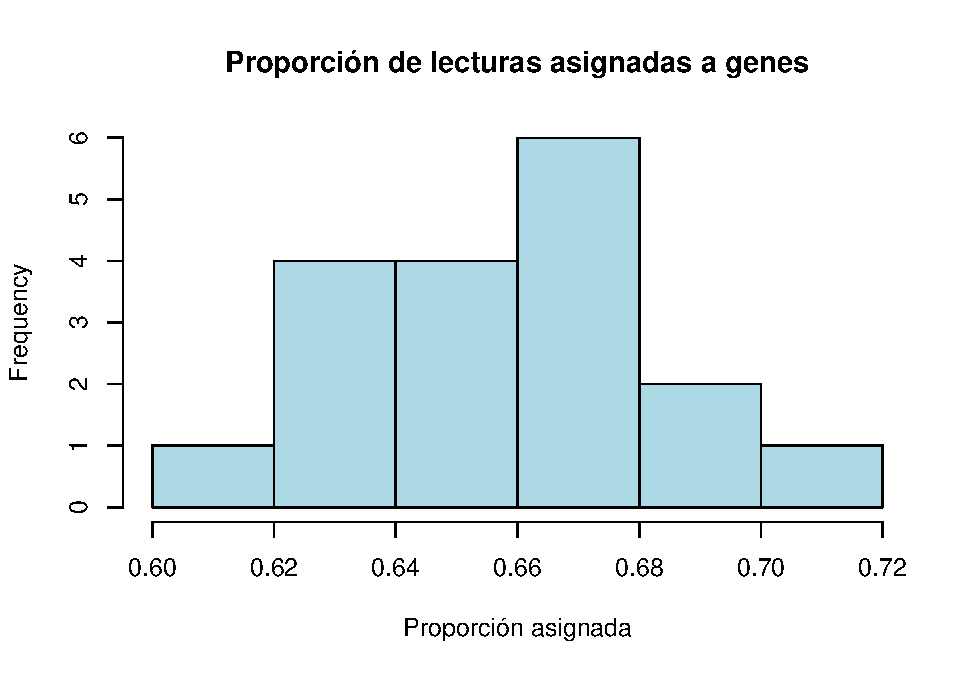
\includegraphics{Proyecto_RNAseq_files/figure-latex/unnamed-chunk-8-1.pdf}

\begin{Shaded}
\begin{Highlighting}[]
\FunctionTok{table}\NormalTok{(rse\_gene\_SRP075398}\SpecialCharTok{$}\NormalTok{assigned\_gene\_prop }\SpecialCharTok{\textless{}} \FloatTok{0.3}\NormalTok{)}
\end{Highlighting}
\end{Shaded}

\begin{verbatim}
## 
## FALSE 
##    18
\end{verbatim}

\begin{Shaded}
\begin{Highlighting}[]
\NormalTok{rse\_gene\_SRP075398 }\OtherTok{\textless{}{-}}\NormalTok{ rse\_gene\_SRP075398[, rse\_gene\_SRP075398}\SpecialCharTok{$}\NormalTok{assigned\_gene\_prop }\SpecialCharTok{\textgreater{}} \FloatTok{0.3}\NormalTok{]}

\CommentTok{\# Filtrar genes de baja expresión usando edgeR}
\NormalTok{dge }\OtherTok{\textless{}{-}} \FunctionTok{DGEList}\NormalTok{(}\AttributeTok{counts =} \FunctionTok{assay}\NormalTok{(rse\_gene\_SRP075398, }\StringTok{"counts"}\NormalTok{))}
\NormalTok{keep }\OtherTok{\textless{}{-}} \FunctionTok{filterByExpr}\NormalTok{(dge, }\AttributeTok{group =}\NormalTok{ rse\_gene\_SRP075398}\SpecialCharTok{$}\NormalTok{sra\_attribute.transfection)}
\NormalTok{rse\_gene\_SRP075398 }\OtherTok{\textless{}{-}}\NormalTok{ rse\_gene\_SRP075398[keep, ]}

\CommentTok{\# Dimensiones finales}
\FunctionTok{dim}\NormalTok{(rse\_gene\_SRP075398)}
\end{Highlighting}
\end{Shaded}

\begin{verbatim}
## [1] 22789    18
\end{verbatim}

\begin{Shaded}
\begin{Highlighting}[]
\CommentTok{\# Porcentaje de genes retenidos}
\FunctionTok{round}\NormalTok{(}\FunctionTok{nrow}\NormalTok{(rse\_gene\_SRP075398) }\SpecialCharTok{/} \FunctionTok{nrow}\NormalTok{(rse\_gene\_SRP075398\_unfiltered) }\SpecialCharTok{*} \DecValTok{100}\NormalTok{, }\DecValTok{2}\NormalTok{)}
\end{Highlighting}
\end{Shaded}

\begin{verbatim}
## [1] 35.69
\end{verbatim}

\subsection{Normalización de los
datos}\label{normalizaciuxf3n-de-los-datos}

\begin{Shaded}
\begin{Highlighting}[]
\CommentTok{\# Crear un objeto DGEList para normalización}
\NormalTok{dge }\OtherTok{\textless{}{-}} \FunctionTok{DGEList}\NormalTok{(}
    \AttributeTok{counts =} \FunctionTok{assay}\NormalTok{(rse\_gene\_SRP075398, }\StringTok{"counts"}\NormalTok{),}
    \AttributeTok{genes =} \FunctionTok{rowData}\NormalTok{(rse\_gene\_SRP075398)}
\NormalTok{)}

\CommentTok{\# Normalización TMM}
\NormalTok{dge }\OtherTok{\textless{}{-}} \FunctionTok{calcNormFactors}\NormalTok{(dge)}

\NormalTok{dge}
\end{Highlighting}
\end{Shaded}

\begin{verbatim}
## An object of class "DGEList"
## $counts
##                   SRR3544525 SRR3544526 SRR3544527 SRR3544528 SRR3544529
## ENSG00000223972.5         44         31         54         44         62
## ENSG00000227232.5        297        264        405        352        242
## ENSG00000238009.6         32         27         19         32         20
## ENSG00000268903.1         17          7          9          6         17
## ENSG00000269981.1         14         19         25         23         16
##                   SRR3544530 SRR3544531 SRR3544532 SRR3544533 SRR3544538
## ENSG00000223972.5         37         51         13         18         16
## ENSG00000227232.5        215        277        200        204        245
## ENSG00000238009.6         15         25         19         30         48
## ENSG00000268903.1          6         13          8          3          4
## ENSG00000269981.1         12         34         20         22         25
##                   SRR3544539 SRR3544523 SRR3544524 SRR3544534 SRR3544535
## ENSG00000223972.5         13         71         52         10         11
## ENSG00000227232.5        105        509        353        217        123
## ENSG00000238009.6         23         45         28         26         31
## ENSG00000268903.1          1         35         24          0          4
## ENSG00000269981.1         10         37         33         17         10
##                   SRR3544536 SRR3544537 SRR3544540
## ENSG00000223972.5          7          9         25
## ENSG00000227232.5         74        163        183
## ENSG00000238009.6         32         27         45
## ENSG00000268903.1          0          2          3
## ENSG00000269981.1          6         13         26
## 22784 more rows ...
## 
## $samples
##            group lib.size norm.factors
## SRR3544525     1 40704527    1.0515272
## SRR3544526     1 44710538    1.0305267
## SRR3544527     1 55789726    0.9938596
## SRR3544528     1 61289070    1.0017792
## SRR3544529     1 34508615    1.0395402
## 13 more rows ...
## 
## $genes
##                   source type bp_length phase           gene_id
## ENSG00000223972.5 HAVANA gene      1735    NA ENSG00000223972.5
## ENSG00000227232.5 HAVANA gene      1351    NA ENSG00000227232.5
## ENSG00000238009.6 HAVANA gene      3726    NA ENSG00000238009.6
## ENSG00000268903.1 HAVANA gene       755    NA ENSG00000268903.1
## ENSG00000269981.1 HAVANA gene       284    NA ENSG00000269981.1
##                                            gene_type     gene_name level
## ENSG00000223972.5 transcribed_unprocessed_pseudogene       DDX11L1     2
## ENSG00000227232.5             unprocessed_pseudogene        WASH7P     2
## ENSG00000238009.6                            lincRNA  RP11-34P13.7     2
## ENSG00000268903.1               processed_pseudogene RP11-34P13.15     2
## ENSG00000269981.1               processed_pseudogene RP11-34P13.16     2
##                            havana_gene               tag
## ENSG00000223972.5 OTTHUMG00000000961.2              <NA>
## ENSG00000227232.5 OTTHUMG00000000958.1              <NA>
## ENSG00000238009.6 OTTHUMG00000001096.2 overlapping_locus
## ENSG00000268903.1 OTTHUMG00000182518.2              <NA>
## ENSG00000269981.1 OTTHUMG00000182738.2              <NA>
## 22784 more rows ...
\end{verbatim}

\subsection{Determinar el modelo
estadístico}\label{determinar-el-modelo-estaduxedstico}

\begin{Shaded}
\begin{Highlighting}[]
\NormalTok{mod }\OtherTok{\textless{}{-}} \FunctionTok{model.matrix}\NormalTok{(}
  \SpecialCharTok{\textasciitilde{}}\NormalTok{ sra\_attribute.cell\_line }\SpecialCharTok{*}\NormalTok{ sra\_attribute.transfection,}
  \AttributeTok{data =} \FunctionTok{colData}\NormalTok{(rse\_gene\_SRP075398)}
\NormalTok{)}

\FunctionTok{colnames}\NormalTok{(mod)}
\end{Highlighting}
\end{Shaded}

\begin{verbatim}
## [1] "(Intercept)"                                                         
## [2] "sra_attribute.cell_lineMCF-7"                                        
## [3] "sra_attribute.transfectionPre-miR-29a"                               
## [4] "sra_attribute.transfectionPre-miR-29b-1"                             
## [5] "sra_attribute.cell_lineMCF-7:sra_attribute.transfectionPre-miR-29a"  
## [6] "sra_attribute.cell_lineMCF-7:sra_attribute.transfectionPre-miR-29b-1"
\end{verbatim}

\begin{Shaded}
\begin{Highlighting}[]
\CommentTok{\# Simplificar nombres de la columna}

\CommentTok{\#colnames(mod) \textless{}{-} c("Intercept", "CellLine\_MCF7", "Transfection\_miR29a", }
                   \CommentTok{\#"Transfection\_miR29b1", "Interaction\_MCF7\_miR29a", }
                   \CommentTok{\#"Interaction\_MCF7\_miR29b1")}
\end{Highlighting}
\end{Shaded}

\section{Visualizar matriz (REVISAR ESTO AL
FINAL)}\label{visualizar-matriz-revisar-esto-al-final}

\begin{Shaded}
\begin{Highlighting}[]
\FunctionTok{library}\NormalTok{(ExploreModelMatrix)}

\DocumentationTok{\#\# Crear las visualizaciones}
\NormalTok{vd }\OtherTok{\textless{}{-}}\NormalTok{ ExploreModelMatrix}\SpecialCharTok{::}\FunctionTok{VisualizeDesign}\NormalTok{(}
    \AttributeTok{sampleData =} \FunctionTok{colData}\NormalTok{(rse\_gene\_SRP075398), }\CommentTok{\# Metadatos de las muestras}
    \AttributeTok{designFormula =} \SpecialCharTok{\textasciitilde{}}\NormalTok{ sra\_attribute.cell\_line }\SpecialCharTok{*}\NormalTok{ sra\_attribute.transfection,           }\CommentTok{\# Fórmula del modelo}
    \AttributeTok{textSizeFitted =} \DecValTok{1}                       \CommentTok{\# Tamaño del texto}
\NormalTok{)}

\FunctionTok{library}\NormalTok{(cowplot)}
\NormalTok{cowplot}\SpecialCharTok{::}\FunctionTok{plot\_grid}\NormalTok{(}\AttributeTok{plotlist =}\NormalTok{ vd}\SpecialCharTok{$}\NormalTok{plotlist)}
\end{Highlighting}
\end{Shaded}

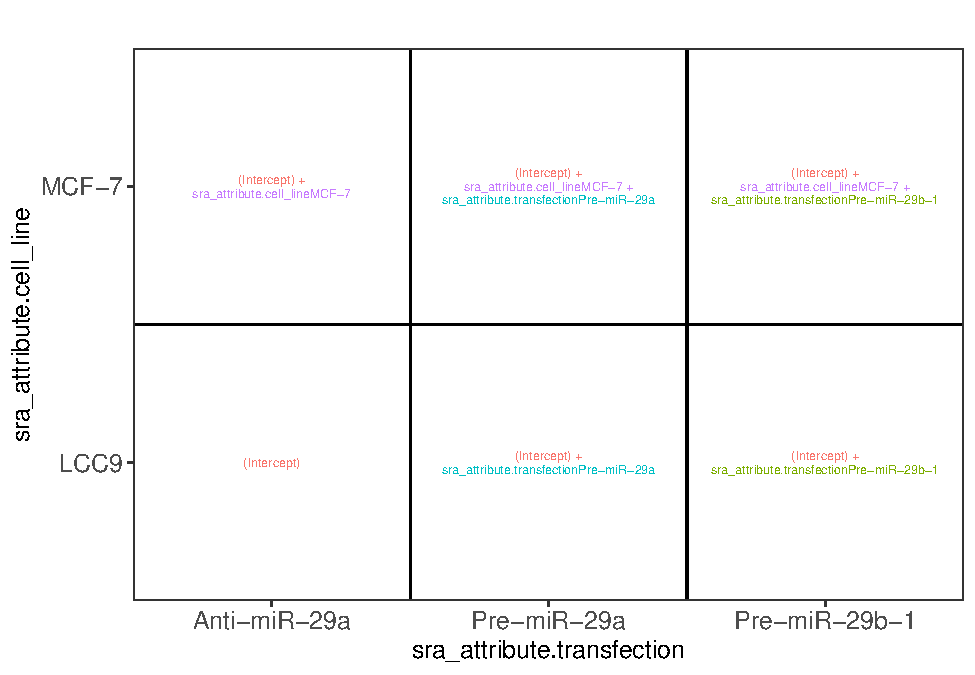
\includegraphics{Proyecto_RNAseq_files/figure-latex/unnamed-chunk-11-1.pdf}

\section{Expresión diferencial}\label{expresiuxf3n-diferencial}

\begin{Shaded}
\begin{Highlighting}[]
\NormalTok{vGene }\OtherTok{\textless{}{-}} \FunctionTok{voom}\NormalTok{(dge, mod, }\AttributeTok{plot =} \ConstantTok{TRUE}\NormalTok{)}
\end{Highlighting}
\end{Shaded}

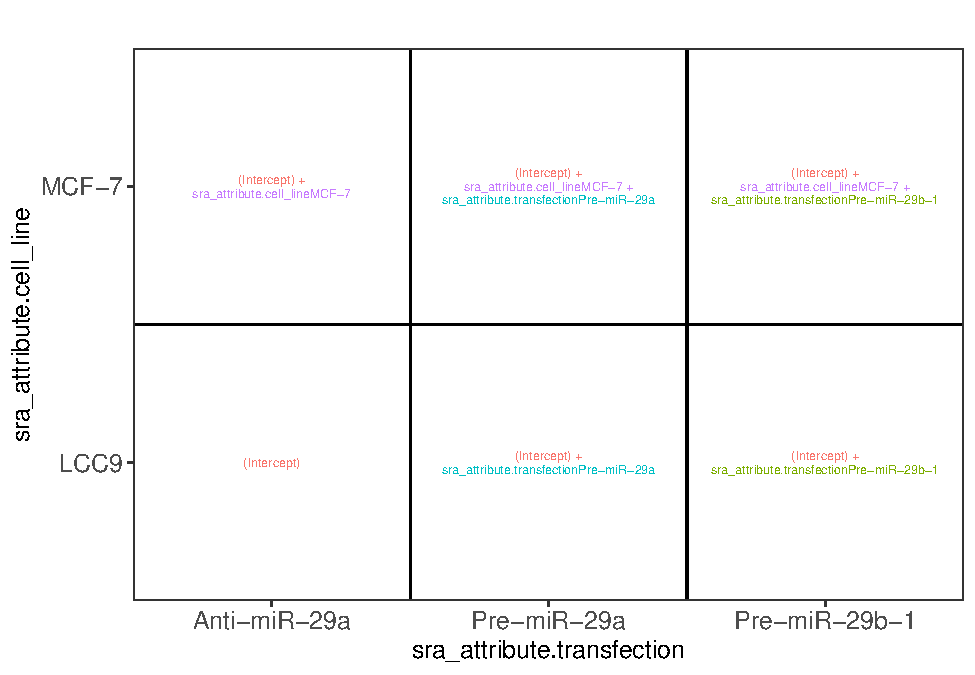
\includegraphics{Proyecto_RNAseq_files/figure-latex/unnamed-chunk-12-1.pdf}

\begin{Shaded}
\begin{Highlighting}[]
\CommentTok{\# Ajuste del modelo lineal y cálculo de estadísticas empíricas de Bayes}
\NormalTok{eb\_results }\OtherTok{\textless{}{-}} \FunctionTok{eBayes}\NormalTok{(}\FunctionTok{lmFit}\NormalTok{(vGene))}

\NormalTok{de\_results }\OtherTok{\textless{}{-}} \FunctionTok{topTable}\NormalTok{(}
\NormalTok{    eb\_results,}
    \AttributeTok{coef =} \DecValTok{2}\NormalTok{,}
    \AttributeTok{number =} \FunctionTok{nrow}\NormalTok{(rse\_gene\_SRP075398),}
    \AttributeTok{sort.by =} \StringTok{"none"}
\NormalTok{)}

\CommentTok{\# Dimensiones y vista preliminar de los resultados}
\FunctionTok{dim}\NormalTok{(de\_results)}
\end{Highlighting}
\end{Shaded}

\begin{verbatim}
## [1] 22789    16
\end{verbatim}

\begin{Shaded}
\begin{Highlighting}[]
\FunctionTok{head}\NormalTok{(de\_results)}
\end{Highlighting}
\end{Shaded}

\begin{verbatim}
##                   source type bp_length phase           gene_id
## ENSG00000223972.5 HAVANA gene      1735    NA ENSG00000223972.5
## ENSG00000227232.5 HAVANA gene      1351    NA ENSG00000227232.5
## ENSG00000238009.6 HAVANA gene      3726    NA ENSG00000238009.6
## ENSG00000268903.1 HAVANA gene       755    NA ENSG00000268903.1
## ENSG00000269981.1 HAVANA gene       284    NA ENSG00000269981.1
## ENSG00000239906.1 HAVANA gene       323    NA ENSG00000239906.1
##                                            gene_type     gene_name level
## ENSG00000223972.5 transcribed_unprocessed_pseudogene       DDX11L1     2
## ENSG00000227232.5             unprocessed_pseudogene        WASH7P     2
## ENSG00000238009.6                            lincRNA  RP11-34P13.7     2
## ENSG00000268903.1               processed_pseudogene RP11-34P13.15     2
## ENSG00000269981.1               processed_pseudogene RP11-34P13.16     2
## ENSG00000239906.1                          antisense RP11-34P13.14     2
##                            havana_gene               tag      logFC    AveExpr
## ENSG00000223972.5 OTTHUMG00000000961.2              <NA> -1.6682397 -0.7347566
## ENSG00000227232.5 OTTHUMG00000000958.1              <NA> -1.0300576  2.4023283
## ENSG00000238009.6 OTTHUMG00000001096.2 overlapping_locus  0.7712042 -0.5755998
## ENSG00000268903.1 OTTHUMG00000182518.2              <NA> -1.6043444 -2.9389997
## ENSG00000269981.1 OTTHUMG00000182738.2              <NA> -0.6971305 -1.1724133
## ENSG00000239906.1 OTTHUMG00000002481.1              <NA>  1.5168961 -0.5286964
##                           t      P.Value    adj.P.Val          B
## ENSG00000223972.5 -4.947936 0.0001334750 0.0002696371  0.8157153
## ENSG00000227232.5 -4.097809 0.0007946777 0.0013918923 -1.7013844
## ENSG00000238009.6  3.158990 0.0059046617 0.0088550498 -3.1137314
## ENSG00000268903.1 -1.811961 0.0882499498 0.1089038883 -4.9948247
## ENSG00000269981.1 -1.625628 0.1229935089 0.1480665121 -5.6956305
## ENSG00000239906.1  3.957787 0.0010712285 0.0018297276 -1.3144976
\end{verbatim}

\begin{Shaded}
\begin{Highlighting}[]
\DocumentationTok{\#\# Genes diferencialmente expresados con FDR \textless{} 5\%}
\FunctionTok{table}\NormalTok{(de\_results}\SpecialCharTok{$}\NormalTok{adj.P.Val }\SpecialCharTok{\textless{}} \FloatTok{0.05}\NormalTok{)}
\end{Highlighting}
\end{Shaded}

\begin{verbatim}
## 
## FALSE  TRUE 
##  5408 17381
\end{verbatim}

\begin{Shaded}
\begin{Highlighting}[]
\DocumentationTok{\#\# Visualizar los resultados estadísticos}

\FunctionTok{plotMA}\NormalTok{(eb\_results, }\AttributeTok{coef =} \DecValTok{2}\NormalTok{)}
\end{Highlighting}
\end{Shaded}

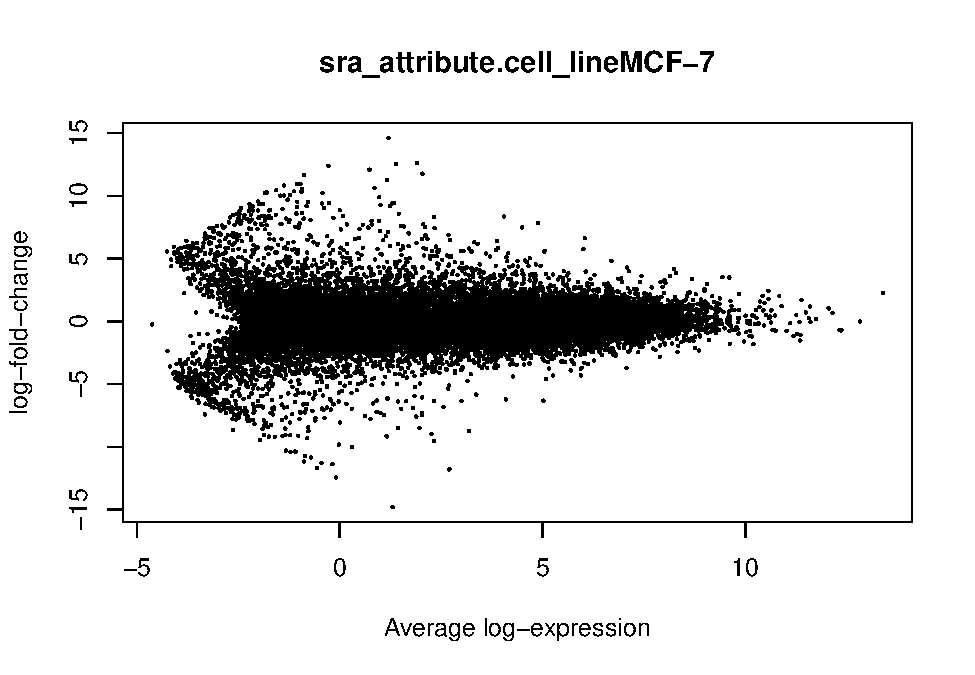
\includegraphics{Proyecto_RNAseq_files/figure-latex/unnamed-chunk-13-1.pdf}

\begin{Shaded}
\begin{Highlighting}[]
\FunctionTok{volcanoplot}\NormalTok{(eb\_results, }\AttributeTok{coef =} \DecValTok{2}\NormalTok{, }\AttributeTok{highlight =} \DecValTok{3}\NormalTok{, }\AttributeTok{names =}\NormalTok{ de\_results}\SpecialCharTok{$}\NormalTok{gene\_name)}
\end{Highlighting}
\end{Shaded}

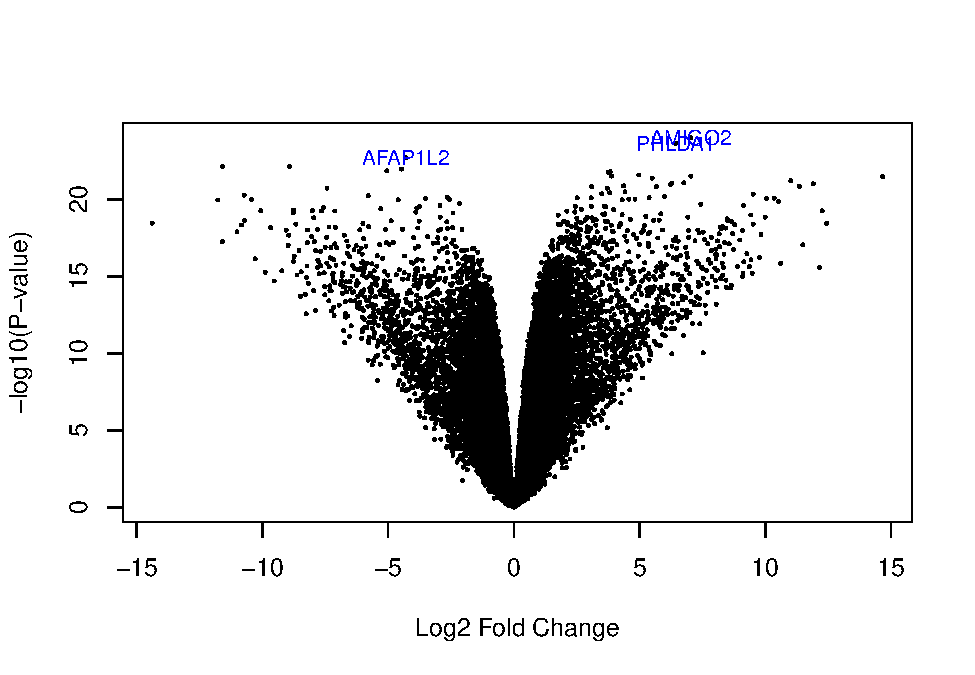
\includegraphics{Proyecto_RNAseq_files/figure-latex/unnamed-chunk-13-2.pdf}

\begin{Shaded}
\begin{Highlighting}[]
\DocumentationTok{\#\# Información de los 3 genes más significativos }
\NormalTok{de\_results[de\_results}\SpecialCharTok{$}\NormalTok{gene\_name }\SpecialCharTok{\%in\%} \FunctionTok{c}\NormalTok{(}\StringTok{"AMIGO2"}\NormalTok{, }\StringTok{"APBB2"}\NormalTok{, }\StringTok{"LGALS3"}\NormalTok{), ]}
\end{Highlighting}
\end{Shaded}

\begin{verbatim}
##                    source type bp_length phase            gene_id
## ENSG00000139211.6  HAVANA gene      3956    NA  ENSG00000139211.6
## ENSG00000131981.15 HAVANA gene      2397    NA ENSG00000131981.15
## ENSG00000163697.16 HAVANA gene     12956    NA ENSG00000163697.16
##                         gene_type gene_name level           havana_gene
## ENSG00000139211.6  protein_coding    AMIGO2     2  OTTHUMG00000169616.1
## ENSG00000131981.15 protein_coding    LGALS3     1  OTTHUMG00000171030.4
## ENSG00000163697.16 protein_coding     APBB2     2 OTTHUMG00000160416.11
##                           tag    logFC  AveExpr        t      P.Value
## ENSG00000139211.6        <NA> 6.619379 6.044395 88.02985 1.804171e-23
## ENSG00000131981.15       <NA> 7.844704 4.895663 60.85097 7.793307e-21
## ENSG00000163697.16 ncRNA_host 7.492499 4.501818 65.39220 2.390532e-21
##                       adj.P.Val        B
## ENSG00000139211.6  4.111525e-19 42.91918
## ENSG00000131981.15 5.145767e-17 36.96864
## ENSG00000163697.16 2.723892e-17 37.95833
\end{verbatim}

\section{Visualizar genes DE}\label{visualizar-genes-de}

\begin{Shaded}
\begin{Highlighting}[]
\CommentTok{\# Revisar los top 50 genes diferencialmente expresados}

\DocumentationTok{\#\# Extraer valores de los genes de interés}
\NormalTok{exprs\_heatmap }\OtherTok{\textless{}{-}}\NormalTok{ vGene}\SpecialCharTok{$}\NormalTok{E[}\FunctionTok{rank}\NormalTok{(de\_results}\SpecialCharTok{$}\NormalTok{adj.P.Val) }\SpecialCharTok{\textless{}=} \DecValTok{50}\NormalTok{, ]}

\DocumentationTok{\#\# Creemos una tabla con información de las muestras}
\DocumentationTok{\#\# y con nombres de columnas más amigables}
\NormalTok{df }\OtherTok{\textless{}{-}} \FunctionTok{as.data.frame}\NormalTok{(}\FunctionTok{colData}\NormalTok{(rse\_gene\_SRP075398)[, }\FunctionTok{c}\NormalTok{(}\StringTok{"sra\_attribute.cell\_line"}\NormalTok{, }\StringTok{"sra\_attribute.transfection"}\NormalTok{)])}
\FunctionTok{colnames}\NormalTok{(df) }\OtherTok{\textless{}{-}} \FunctionTok{c}\NormalTok{(}\StringTok{"Cell\_line"}\NormalTok{, }\StringTok{"Transfection"}\NormalTok{)}

\DocumentationTok{\#\# Hagamos un heatmap}
\FunctionTok{library}\NormalTok{(}\StringTok{"pheatmap"}\NormalTok{)}
\FunctionTok{pheatmap}\NormalTok{(}
\NormalTok{    exprs\_heatmap,}
    \AttributeTok{cluster\_rows =} \ConstantTok{TRUE}\NormalTok{,}
    \AttributeTok{cluster\_cols =} \ConstantTok{TRUE}\NormalTok{,}
    \AttributeTok{show\_rownames =} \ConstantTok{FALSE}\NormalTok{,}
    \AttributeTok{show\_colnames =} \ConstantTok{FALSE}\NormalTok{,}
    \AttributeTok{annotation\_col =}\NormalTok{ df}
\NormalTok{)}
\end{Highlighting}
\end{Shaded}

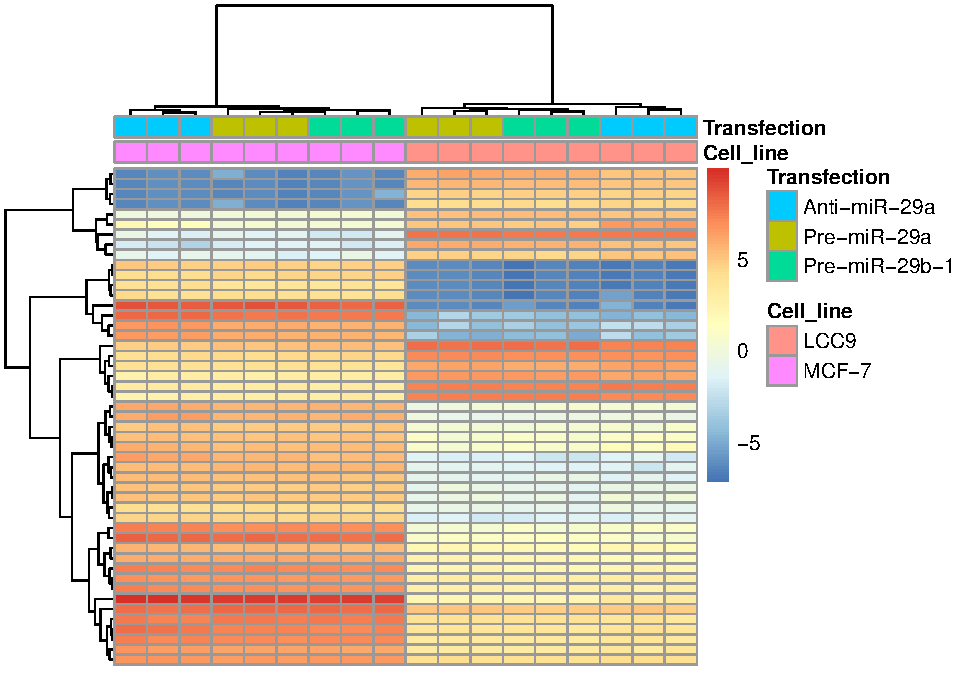
\includegraphics{Proyecto_RNAseq_files/figure-latex/unnamed-chunk-14-1.pdf}

\begin{Shaded}
\begin{Highlighting}[]
\CommentTok{\# MDS (multidimensional scaling)}

\DocumentationTok{\#\# Para colores}
\FunctionTok{library}\NormalTok{(}\StringTok{"RColorBrewer"}\NormalTok{)}

\DocumentationTok{\#\# Conviertiendo los grupos de Cell\_line a colores}
\NormalTok{col.group }\OtherTok{\textless{}{-}}\NormalTok{ df}\SpecialCharTok{$}\NormalTok{Cell\_line}
\FunctionTok{levels}\NormalTok{(col.group) }\OtherTok{\textless{}{-}} \FunctionTok{brewer.pal}\NormalTok{(}\FunctionTok{nlevels}\NormalTok{(col.group), }\StringTok{"Set1"}\NormalTok{)}
\end{Highlighting}
\end{Shaded}

\begin{verbatim}
## Warning in brewer.pal(nlevels(col.group), "Set1"): minimal value for n is 3, returning requested palette with 3 different levels
\end{verbatim}

\begin{Shaded}
\begin{Highlighting}[]
\NormalTok{col.group }\OtherTok{\textless{}{-}} \FunctionTok{as.character}\NormalTok{(col.group)}

\DocumentationTok{\#\# MDS por grupos de Cell\_line}
\FunctionTok{plotMDS}\NormalTok{(vGene}\SpecialCharTok{$}\NormalTok{E, }\AttributeTok{labels =}\NormalTok{ df}\SpecialCharTok{$}\NormalTok{Cell\_line, }\AttributeTok{col =}\NormalTok{ col.group)}
\end{Highlighting}
\end{Shaded}

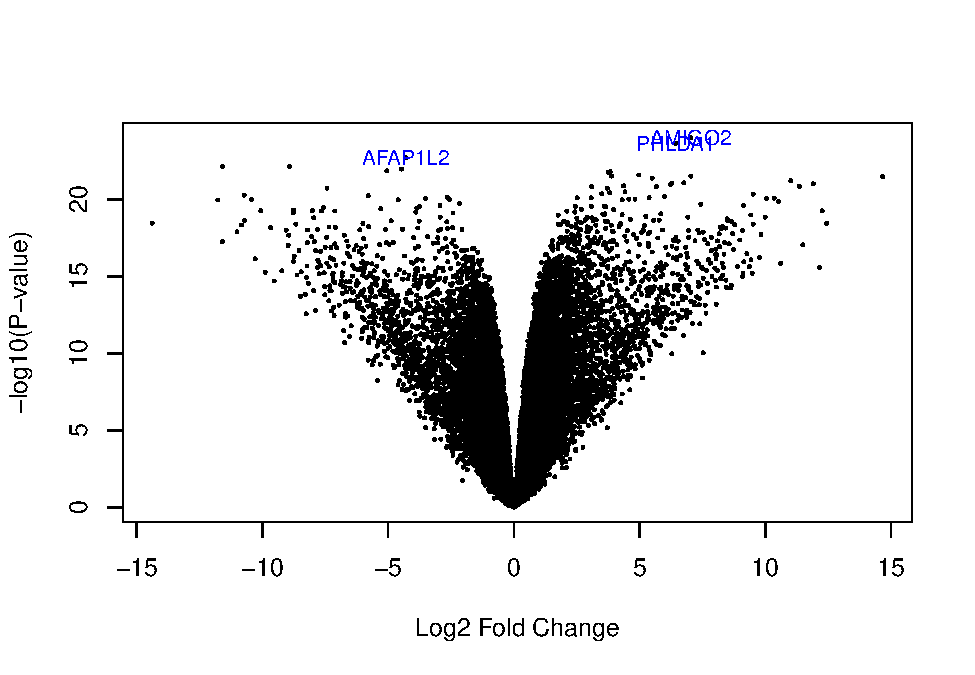
\includegraphics{Proyecto_RNAseq_files/figure-latex/unnamed-chunk-15-1.pdf}

\begin{Shaded}
\begin{Highlighting}[]
\DocumentationTok{\#\# Para colores}
\FunctionTok{library}\NormalTok{(}\StringTok{"RColorBrewer"}\NormalTok{)}

\DocumentationTok{\#\# Convertir Transfection a colores}
\NormalTok{col.group }\OtherTok{\textless{}{-}}\NormalTok{ df}\SpecialCharTok{$}\NormalTok{Transfection}
\NormalTok{df}\SpecialCharTok{$}\NormalTok{Transfection }\OtherTok{\textless{}{-}} \FunctionTok{as.factor}\NormalTok{(df}\SpecialCharTok{$}\NormalTok{Transfection) }\CommentTok{\# Asegúrate de que sea un factor}
\NormalTok{colors }\OtherTok{\textless{}{-}} \FunctionTok{brewer.pal}\NormalTok{(}\FunctionTok{nlevels}\NormalTok{(df}\SpecialCharTok{$}\NormalTok{Transfection), }\StringTok{"Set1"}\NormalTok{) }\CommentTok{\# Generar paleta de colores}
\FunctionTok{levels}\NormalTok{(col.group) }\OtherTok{\textless{}{-}}\NormalTok{ colors }\CommentTok{\# Asignar colores a los niveles}
\NormalTok{col.group }\OtherTok{\textless{}{-}} \FunctionTok{as.character}\NormalTok{(col.group) }\CommentTok{\# Convertir a vector de caracteres}

\DocumentationTok{\#\# MDS por grupos de Transfection}
\FunctionTok{plotMDS}\NormalTok{(vGene}\SpecialCharTok{$}\NormalTok{E, }\AttributeTok{labels =}\NormalTok{ df}\SpecialCharTok{$}\NormalTok{Transfection, }\AttributeTok{col =}\NormalTok{ col.group, }
        \AttributeTok{main =} \StringTok{"MDS Plot by Transfection"}\NormalTok{, }\AttributeTok{pch =} \DecValTok{16}\NormalTok{)}

\DocumentationTok{\#\# Agregar leyenda}
\FunctionTok{legend}\NormalTok{(}\StringTok{"topright"}\NormalTok{, }\AttributeTok{legend =} \FunctionTok{levels}\NormalTok{(df}\SpecialCharTok{$}\NormalTok{Transfection), }\AttributeTok{fill =} \FunctionTok{unique}\NormalTok{(col.group),}
       \AttributeTok{title =} \StringTok{"Transfection Groups"}\NormalTok{)}
\end{Highlighting}
\end{Shaded}

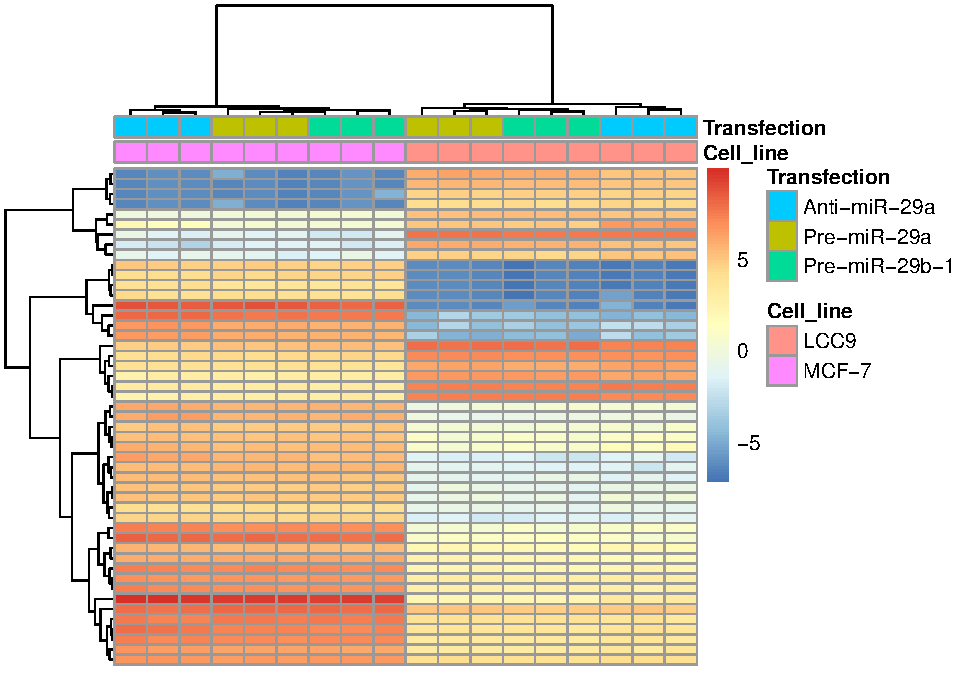
\includegraphics{Proyecto_RNAseq_files/figure-latex/unnamed-chunk-16-1.pdf}

\end{document}
